\chapter{Spezifische Elektronenladung e/m}
\label{v:20}

In diesem Versuch wird die historische Messung der spezifischen Elektronenladung (fast originalgetreu) nachvollzogen. Dabei lernen Sie Techniken moderner Teilchenbeschleuniger und Massenspektrometer kennen.

\begin{hint}
Eine der ersten Messungen der spezifischen Elektronenladung gelang Johann Emil Wiechert , der das Elektron etwa zeitgleich mit Joseph John Thompson entdeckte, der dafür den Nobelpreis erhielt.\\ 
Wiechert arbeitete ab 1897 an der Universität Göttingen und erhielt hier 1898 den Ruf auf die weltweit erste Professur für Geophysik.
\end{hint}

%------------------------------------------------
\section{Stichworte}
%------------------------------------------------

Erzeugung eines homogenen Magnetfeldes; Helmholtz-Spulen; Lorentzkraft; Bewegung geladener Teilchen in elektrischen und magnetischen Feldern.
%
%------------------------------------------------
\section{Literatur}
%------------------------------------------------

Gehrtsen, Kapitel 7.1.2/3 und 8.2.1/2
%
%------------------------------------------------
\section{Anwendungsbeispiele}
%------------------------------------------------

Die Messung der spezifischen Elektronenladung, die J.J. Thomson zuerst in 1897 durchführte, ist einer der größten Meilensteine in der Entdeckung der elementaren Bausteine der Materie. Die Idee, daß Atome nicht unteilbar sind, sondern vielmehr aus grundlegenderen, sogenannten fundamentalen, Bausteinen aufgebaut seien, existierte schon vor Thomsons Messungen. Allerdings war die Annahme, daß diese Bausteine dieselbe Größe hätten, wie das kleinste bekannte Atome, das Wasserstoffatome. Basierend auf seiner Beobachtung, daß Kathodenstrahlen eine sehr viel größere Reichweite in Luft haben, als für ein Teilchen von der Größe eines Atoms zu erwarten war, schlug Thomson die Existenz eines fundamentalen Teilchens vor, welches mehr als tausendmal kleiner sei als ein Wasserstoffatom.\\
In seinem Experiment zur Messung der spezifischen Ladung der Teilchen, die die Kathodenstrahlen ausmachten fand er, daß diese sogar etwa 2000 mal größer ist, als die für ein H-Atom erwartete. Nach der Messung der Ladung dieser Teilchen im Millikan Versuch war klar, daß diese Teilchen zwar dieselbe Ladung (bis auf das Vorzeichen) wie ein H-Atomkern haben, aber etwa 2000 mal leichter sind, was die große Reichweite in Luft erklärte. Weiterhin konnte Thomson zeigen, daß Kathodenstrahlen immer aus eben diesen Teilchen bestehen, unabhängig vom Material der Kathode von der sie ausgestrahlt werden.\\
Diese Ergebnisse, die seit langem zu unserem Schulbuchwissen gehören, brachten Thomson den Nobelpreis in 1906 ein und machten ihn allgemein bekannt als den Entdecker des Elektrons.

\noindent
Die von Thomson benutze Technik, geladene Teilchen in elektrischen Feldern zu beschleunigen und in magnetischen Felder abzulenken, wird heute nicht nur in modernen Teilchenbeschelunigern in der Grundlagenphysik, der medizinischen Hadronen- und Strahlentherapie und der Materialprüfung eingesetzt, sondern wird auch in Massenspektrometern benutzt, um chemische Verbindungen zu charakterisieren. Beispiele hierfür sind die Identifizierung von Substanzen in Körperflüssigkeiten in der medizinischen Chemie, kriminaltechnische Untersuchungen, Dopingkontrolle und die militärische Analytik von chemischen Kampfstoffen.

%------------------------------------------------
\section{Theoretischer Hintergrund}
%------------------------------------------------

\subsection{Bewegung geladener Teilchen in E- und B-Feldern}

Geladene Teilchen werden von elektrischen und magnetischen Feldern unvergleichlich viel stärker beeinflusst als vom Gravitationsfeld (außer in der Nähe schwarzer Löcher). 

\subsubsection*{Geladene Teilchen im homogenen elektrischen Feld}

Zwischen zwei planparallelen Platten mit dem Abstand $D$ im Vakuum liege die Spannung $U$. Wenn keine Ladungsträger zwischen den Platten das Feld verzerren, ist dieses homogen und hat die Form $\vec{E}=\frac{U}{d}\vec{e}_E$. Dieses Feld übt auf eine elektrische Ladung $Q$, welche wir in Einheiten der Ladung des Elektrons (Elementarladung) angeben als $Q = q\cdot e$, eine Kraft $\vec{F} = qe\vec{E}$ aus und beschleunigt sie mit
\begin{equation}
	\vec{a} = \frac{qe}{m}\frac{U}{d}\vec{e}_E\; .
\end{equation}
Wie man sieht, wirkt die Kraft immer in Richtung des elektrischen Feldes. Elektrische Felder können also sowohl zur Umlenkung geladener Teilchen benutzt werden, als auch zur Beschleunigung (i.e. Erhöhung der kinetischen Energie).

\subsubsection*{Geladene Teilchen im homogenen Magnetfeld}

Wenn eine Ladung $Q = q\cdot e$ mit der Geschwindigkeit $\vec{v}$ durch ein Magnetfeld $\vec{B}$ fliegt, so erfährt sie eine Kraft 
\begin{equation}
	\vec{F} = qe\, \vec{v}\times\vec{B}\, ,
\end{equation}
die Lorentz-Karft. Diese steht, wie man am Kreuzprodukt sieht (Rechte-Hand-Regel), senkrecht auf der Bewegungsrichtung und der magnetischen Feldrichtung. Magnetfelder können damit nur zur Umlenkung geladener Teilchen benutzt werden, nicht jedoch zur Erhöhung der kinetischen Energie des Teilchens.

%------------------------------------------------
\section{Versuchsaufbau}
%------------------------------------------------

\begin{minipage}{.35\textwidth}
Das nebenstehende Bild zeigt ein Foto des Versuches mit Zubehör: Fadenstrahlrohr mit Helmholtzspule und verschiebbarer Ablesevorrichtung, Steuerung für Fadenstrahlrohr (im wesentlichen Netzgerät für Kathodenheizung, Wehneltzylinder und Anodenspannung), Netzgerät mit regelbarem Strom für die Helmholtz-Spule, 2-3 Multimeter.
\end{minipage}
%
\begin{minipage}{.65\textwidth}
	\begin{center}
		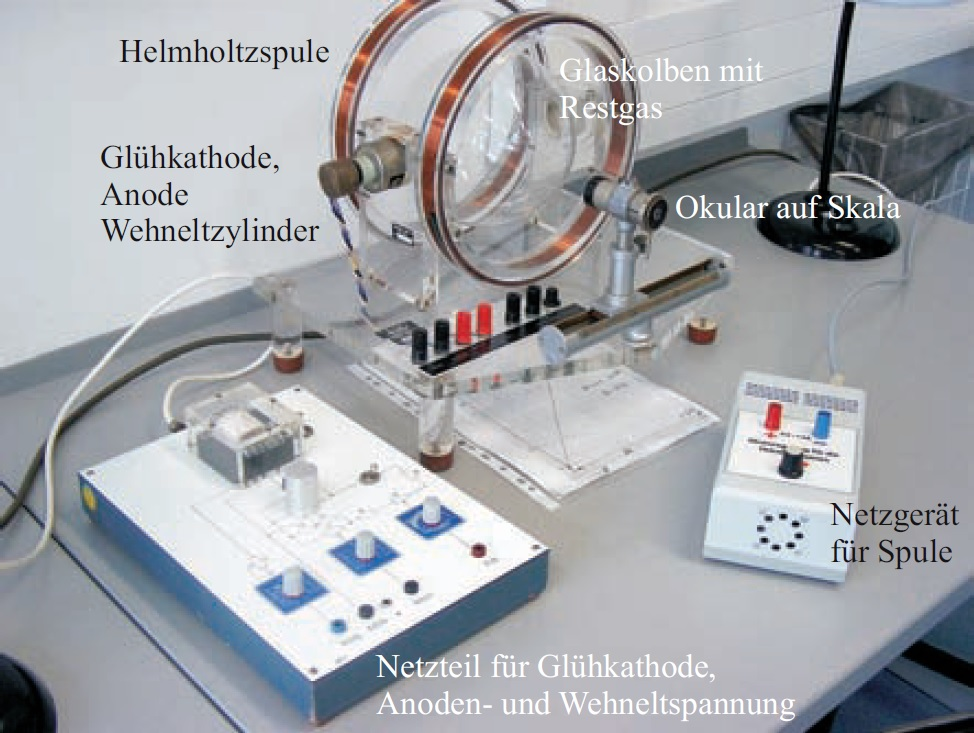
\includegraphics[width=0.90\textwidth]{Abbildungen/em_Aufbau.jpg}
	\end{center}
\end{minipage}


\etutorhint{
	Das Fadenstrahlrohr ist drehbar um seine Längsachse. Das bedeutet, dass die Richtung des Elektronenstrahls bzgl. der Richtung des Magnetfeldes eingestellt werden kann. Wenn der Elektronenstrahl nicht senkrecht zum Magnetfeld steht, so erfährt er nicht nur eine Ablenkung auf die Kreisbahn, sondern behält zusätzlich eine Geschwindigkeitskomponente in Richtung des Magnetfeldes. Da auf diese keine Kraft wirkt, bleibt sie erhalten und führt dazu, dass der Strahl keine reine Kreisbahn bildet, sondern eine Spirale.\\
	Um das zu korrigieren kann das Fadenstrahlrohr per Hand so ausgerichtet werden, dass der Strahl wieder senkrecht zum Magnetfeld steht.
}
%------------------------------------------------
\section{Fragen zur Vorbereitung}
%------------------------------------------------

\begin{enumerate}
	%
%	\item Was soll heute im Praktikum gemessen werden? Warum?
	%
	\item Wie lautet der Ausdruck für die Kraft zwischen zwei Punktladungen?
	%
	\item Wie berechnet sich das elektrische Feld eines Plattenkondensators aus der Spannung $U$ und dem Plattenabstand $d$?
	%
	\item Welche Geschwindigkeit hat ein Teilchen, wenn es eine Spannung $U$ durchläuft?
	%
	\item Was ist die Lorentz-Kraft? Wie ist sie definiert?
	%
	\item Wie sieht die Bahnkurve eines geladenen Teilchens aus, wenn es sich senkrecht zu einem Magnetfeld bewegt?
	%
	\item Was ist ein homogenes Magnetfeld?
	%
	\item Wie lautet der Ausdruck für die Zentrifugalkraft?
	%
	\item Wie berechnet sich aus Zentrifugalkraft und Lorentzkraft ein Ausdruck für die Spezifische Elektronenladung $e/m$?
	%
\end{enumerate}

%------------------------------------------------
\section{Durchführung} 
%------------------------------------------------

Ein Elektronenstrahl beschreibt im Magnetfeld $B$ zweier Helmholtzspulen eine Kreisbahn. Die Spulen werden wie in der Abbildung unten verschaltet.

\begin{figure}[h]
	\centering
		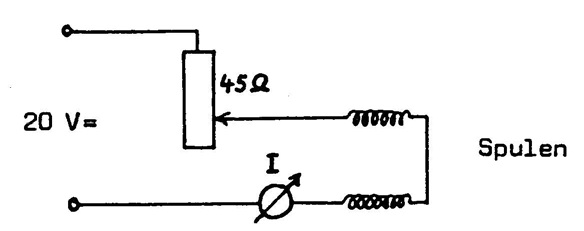
\includegraphics[width=0.50\textwidth]{Abbildungen/Schaltung-HHSpulen.jpg}
	\label{fig:Schaltung-HHSpulen}
\end{figure}

\begin{hint}
Lassen Sie Ihre Schaltung vor dem Einschalten durch den Betreuer überprüfen. Schalten Sie die Anodenspannung erst ein, wenn der Kathodenzylinder rot glüht.
\end{hint}

\noindent
Messen Sie für verschiedene Anodenspannungen: $U$ = (125, 150, ..., 225\,V) und Spulenstromstärken: $I$ = (0.6, 0.7, ..., 0.9\,A) den maximalen Durchmesser $d$ dieser Kreisbahn. Berechnen Sie für einen Messpunkt $e/m$ nach untenstehender Formel.

%------------------------------------------------
\section{Auswertung} 
%------------------------------------------------
\etodo{Musterauswertung}
\begin{enumerate}
	%
	\item Leiten Sie die Gleichung her:
		\begin{equation}
			\frac{U}{B^2} = \frac{er^2}{2m}
		\end{equation}
		Nehmen Sie das Magnetfeld $B$ dabei als konstant an.
	%
	\item Tragen Sie $U/B^2$ als Funktion von $r^2/2$ graphisch auf. Berechnen Sie aus der Steigung der Geraden durch die Messpunkte die spezifische Elektronenladung $e/m$ inklusive Fehler.
\end{enumerate}

\begin{hint}
Zwischen dem Magnetfeld $B$ und dem Spulenstrom $I$ besteht ein linearer Zusammenhang. Die graphische Darstellung der Funktion $B$ = f($I$) für das benutzte Spulenpaar befindet sich auf der nächsten Seite !!
\end{hint}

\etodo{Kann man diese Eichung etwas genauer angeben? Nachmessen oder berechnen!}
\begin{figure}[hb]
	\centering
		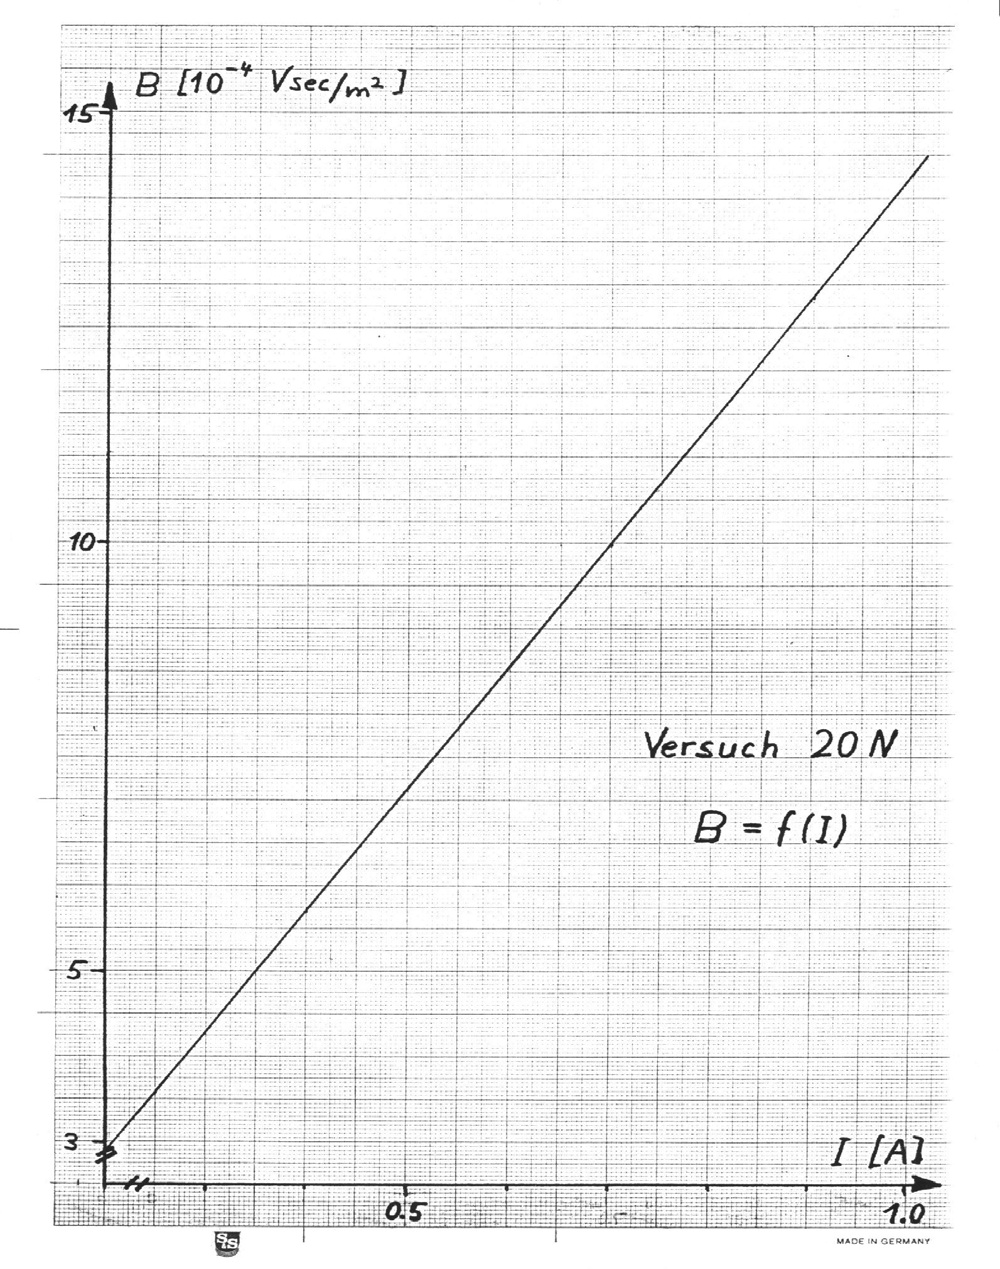
\includegraphics[width=\textwidth]{Abbildungen/Eichung-HHSpulen.jpg}
	\label{fig:Eichung-HHSpulen}
\end{figure}
